% The data remember the recommender -- final presentation
% Build: pdflatex main.tex (twice). Numbers come from numbers.tex (generated by analysis/make_numbers.py).
\documentclass[aspectratio=169,10pt]{beamer}
\usepackage[T1]{fontenc}
\usepackage{lmodern}
\usepackage{microtype}
\usepackage{amsmath,amssymb}
\usepackage{booktabs,array,multirow}
\usepackage{graphicx}
\usepackage{tikz}
\usetikzlibrary{arrows.meta,positioning,calc}
\usepackage{appendixnumberbeamer}
\usepackage{hyperref}

\title{The data remember the recommender}
\author{Dimitris Ntallas \& Orest Mykhailiuk}
\hypersetup{pdftitle={The data remember the recommender: do click models survive a change of recommendation policy?},pdfauthor={Dimitris Ntallas, Orest Mykhailiuk}}

\definecolor{ink}{HTML}{1C3046}
\definecolor{muted}{HTML}{617386}
\definecolor{teal}{HTML}{008C9E}
\definecolor{amber}{HTML}{C27C0E}
\definecolor{plum}{HTML}{8E55C4}
\definecolor{bts}{HTML}{5163C4}
\definecolor{rnd}{HTML}{D04A3A}
\definecolor{pale}{HTML}{EEF5F6}
\definecolor{cloud}{HTML}{F4F6F9}
\definecolor{gridc}{HTML}{E3E8EE}

\setbeamercolor{normal text}{fg=ink,bg=white}
\setbeamercolor{frametitle}{fg=ink,bg=white}
\setbeamercolor{structure}{fg=teal}
\setbeamercolor{block title}{fg=white,bg=ink}
\setbeamercolor{block body}{fg=ink,bg=cloud}
\setbeamertemplate{blocks}[rounded][shadow=false]
\setbeamertemplate{navigation symbols}{}
\setbeamertemplate{itemize item}{\color{teal}\small$\blacktriangleright$}
\setbeamertemplate{itemize subitem}{\color{muted}--}
\setbeamertemplate{enumerate item}{\color{teal}\bfseries\insertenumlabel.}
\setbeamerfont{frametitle}{size=\large,series=\bfseries}
\setbeamertemplate{frametitle}{\vspace{.28cm}\insertframetitle\par\vspace{.04cm}{\color{teal}\rule{1.2cm}{2pt}}\par\vspace{-.05cm}}
\setbeamertemplate{footline}{\hfill\raisebox{.22cm}{\scriptsize\color{muted}\insertframenumber\,/\,\inserttotalframenumber\hspace{.5cm}}}
\setbeamersize{text margin left=.75cm,text margin right=.75cm}
\setlength{\parskip}{0pt}

\newcommand{\take}[1]{\par\vspace{.12cm}{\setlength{\fboxsep}{5pt}\colorbox{pale}{\parbox{\dimexpr\linewidth-2\fboxsep}{\textbf{#1}}}}\par}
\newcommand{\aside}[1]{{\footnotesize\color{muted}#1}}
\newcommand{\bignum}[1]{{\LARGE\bfseries #1}}
\newcommand{\hl}[1]{{\color{teal}\bfseries #1}}
\newcommand{\sect}[1]{{\color{teal}\scriptsize\bfseries\MakeUppercase{#1}}\par\vspace{.05cm}}
\graphicspath{{figures/}}
\newcommand{\btsN}{12.36m}
\newcommand{\rndN}{1.37m}
\newcommand{\btsClicks}{61{,}208}
\newcommand{\rndClicks}{4{,}768}
\newcommand{\btsCTR}{0.495}
\newcommand{\rndCTR}{0.347}
\newcommand{\btsTopTen}{59}
\newcommand{\rndTopTen}{13}
\newcommand{\corrShareCTR}{0.72}
\newcommand{\posCTRa}{0.49}
\newcommand{\posCTRb}{0.50}
\newcommand{\posCTRc}{0.49}
\newcommand{\profShareB}{35.3}
\newcommand{\profShareR}{35.4}
\newcommand{\profLiftB}{1.10}
\newcommand{\profLiftR}{1.17}
\newcommand{\profCTRR}{0.38}
\newcommand{\btsTestCTR}{0.505}
\newcommand{\naivePred}{1.8}
\newcommand{\naiveDiff}{\(-\)29.9}
\newcommand{\naiveRatio}{49}
\newcommand{\ctxRidgeR}{\(-\)0.61}
\newcommand{\ctxRidgeSeen}{\(-\)1.02}
\newcommand{\ridgeC}{1000}
\newcommand{\cartLeaves}{1{,}557}
\newcommand{\forestB}{300}
\newcommand{\forestMf}{10}
\newcommand{\forestLeafText}{min.\ leaf \(\approx\)26 impressions}
\newcommand{\forestGrid}{21}
\newcommand{\fmrBTS}{+3.1}
\newcommand{\fmrBTSci}{+2.5, +3.7}
\newcommand{\fmrRND}{\(-\)0.6}
\newcommand{\fmrRNDci}{\(-\)1.3, +0.1}
\newcommand{\ctxCartB}{+4.0}
\newcommand{\ctxForestB}{+4.6}
\newcommand{\ctxRangeR}{\(-\)1.0 to \(-\)0.4}
\newcommand{\ctxRangeSeen}{\(-\)1.0 to \(-\)0.1}
\newcommand{\finLLB}{0.0311}
\newcommand{\finLLR}{0.0230}
\newcommand{\finSkillB}{\(-\)1.9}
\newcommand{\finSkillR}{\(-\)1.6}
\newcommand{\finAUCB}{0.624}
\newcommand{\finAUCR}{0.610}
\newcommand{\finMeanR}{0.366}
\newcommand{\finTopPredR}{0.84}
\newcommand{\finTopObsR}{0.58}
\newcommand{\finVsSimpleB}{+4.7}
\newcommand{\finVsSimpleBci}{+4.1, +5.3}
\newcommand{\finVsSimpleR}{\(-\)1.2}
\newcommand{\finVsSimpleRci}{\(-\)1.8, \(-\)0.6}
\newcommand{\itemSpread}{3.6}
\newcommand{\posEffect}{2.5}
\newcommand{\posORs}{1.025, 0.998, 0.977}
\newcommand{\curveBTStext}{the trees keep pulling away from ridge as data grow (1m \(\to\) 8.66m: forest improves by 3.0, ridge by 0.3).}
\newcommand{\curveRNDtext}{every model improves too (by 1.3 to 3.5), but at 8.66m all models and the item\(\times\)position table lie within 0.6 of each other.}


\begin{document}

% ---------------------------------------------------------------- 1 TITLE
{\setbeamercolor{background canvas}{bg=ink}
\begin{frame}[plain]
\vspace{.6cm}
{\color{teal}\rule{1.6cm}{3pt}}\par\vspace{.5cm}
{\fontsize{30}{34}\selectfont\color{white}\bfseries The data remember\\[.12cm] the recommender}\par\vspace{.45cm}
{\Large\color{white!80} Do click models survive a change of recommendation policy?}\par
\vfill
{\color{white}Dimitris Ntallas \& Orest Mykhailiuk}\par\vspace{.06cm}
{\small\color{white!65} Statistical and Machine Learning \textperiodcentered{} WU Vienna \textperiodcentered{} ZOZOTOWN Open Bandit Dataset}\par\vspace{.5cm}
\end{frame}}

% ---------------------------------------------------------------- 2 MOTIVATION
\begin{frame}{Every marketplace learns from data its own recommender chose}
\vspace{.15cm}
\begin{columns}[T,onlytextwidth]
\column{.52\linewidth}
Picture a \textbf{service marketplace} that matches customers with providers (doctors, freelancers, tutors). Each visit, the app picks a few providers to show, and we log who gets clicked.\par\vspace{.25cm}
A click model trained on those logs only ever saw what the \emph{old} algorithm chose to show.\par\vspace{.25cm}
\textbf{Then we change the ranking algorithm.}\par\vspace{.1cm}
Can we still trust the click model?
\column{.44\linewidth}
\vspace{-.1cm}
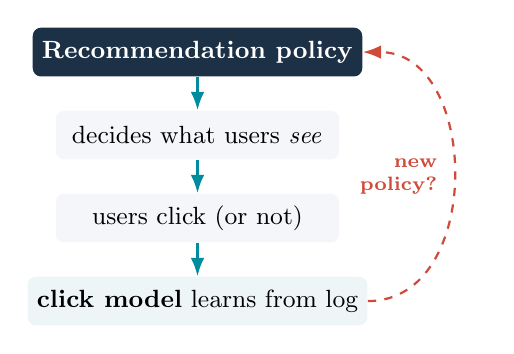
\begin{tikzpicture}[>=Latex,node distance=.42cm,
  box/.style={rounded corners=3pt,fill=cloud,minimum width=3.6cm,minimum height=.62cm,align=center,font=\small}]
\node[box,fill=ink,text=white] (p) {\textbf{Recommendation policy}};
\node[box,below=of p] (s) {decides what users \emph{see}};
\node[box,below=of s] (c) {users click (or not)};
\node[box,below=of c,fill=pale] (m) {\textbf{click model} learns from log};
\draw[->,thick,teal] (p)--(s); \draw[->,thick,teal] (s)--(c); \draw[->,thick,teal] (c)--(m);
\draw[->,thick,rnd,dashed] (m.east) to[out=0,in=0,looseness=1.2] node[left,font=\scriptsize\bfseries,text=rnd,align=right,xshift=-2pt]{new\\policy?} (p.east);
\end{tikzpicture}
\end{columns}
\vspace{.35cm}
\begin{columns}[T,onlytextwidth]
\column{.48\linewidth}
\begin{block}{Q1 \textperiodcentered{} Transfer}
Does a click model trained under one policy stay accurate under another?
\end{block}
\column{.48\linewidth}
\begin{block}{Q2 \textperiodcentered{} What travels}
Which ingredients survive the switch: model flexibility, user context, more data?
\end{block}
\end{columns}
\end{frame}

% ---------------------------------------------------------------- 3 DATA
\begin{frame}{A natural experiment: same shop, same week, two policies}
\vspace{.1cm}
\begin{columns}[T,onlytextwidth]
\column{.50\linewidth}
\textbf{ZOZOTOWN} (Japan's largest fashion e-shop) ran an \textbf{A/B test}: each user impression was randomly served by one of two recommenders.\par\vspace{.25cm}
\renewcommand{\arraystretch}{1.3}
\begin{tabular}{@{}l>{\raggedleft\arraybackslash}p{2.0cm}>{\raggedleft\arraybackslash}p{2.0cm}@{}}
 & {\color{bts}\textbf{BTS}} & {\color{rnd}\textbf{Random}}\\\midrule
Policy & adaptive & uniform\\
Impressions & \btsN & \rndN\\
Clicks & \btsClicks & \rndClicks\\
Click-through rate & \btsCTR\% & \rndCTR\%\\\bottomrule
\end{tabular}\par\vspace{.2cm}
\aside{BTS = Bernoulli Thompson Sampling: shows items that earned clicks before. \quad Campaign ``All'', Nov 2019.}
\column{.45\linewidth}
\sect{Prediction task}
Binary classification:\\[.1cm]
\centerline{\small$P(\text{click}=1 \mid \text{item},\ \text{position},\ \text{user profile})$}\par\vspace{.15cm}
\begin{itemize}\setlength{\itemsep}{2pt}
\item 80 items \textperiodcentered{} 3 slots \textperiodcentered{} 4 anonymised user features
\item \textbf{1 click per 200 impressions} \(\Rightarrow\) we must predict \emph{probabilities}, not labels
\end{itemize}\vspace{.2cm}
\sect{Our rule}
Learn \textbf{only from BTS}. Random plays ``the future after the switch'' and is used only for evaluation, never for fitting or tuning.
\end{columns}
\end{frame}

% ---------------------------------------------------------------- 4 EDA exposure
\begin{frame}{EDA \textperiodcentered{} Thompson sampling shows the winners}
\begin{columns}[T,onlytextwidth]
\column{.60\linewidth}
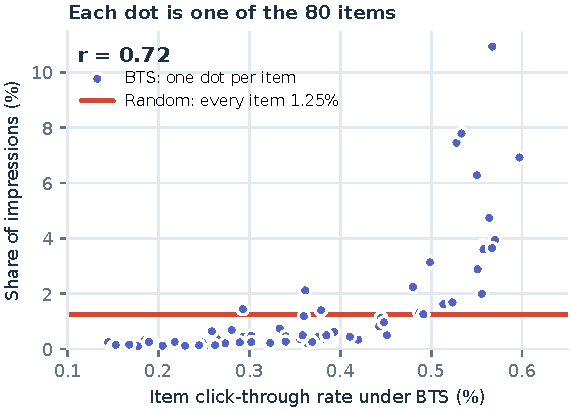
\includegraphics[width=\linewidth,height=.66\textheight,keepaspectratio]{eda_exposure.pdf}
\column{.36\linewidth}
\vspace{.3cm}
\bignum{\btsTopTen\%}\par\aside{of BTS impressions go to its 10 most-shown items (Random: \rndTopTen\%)}\par\vspace{.35cm}
\bignum{r = \corrShareCTR}\par\aside{between an item's click rate and how often BTS shows it}\par\vspace{.35cm}
\bignum{\posCTRa\,/\,\posCTRb\,/\,\posCTRc\%}\par\aside{BTS click rate in slots 1\,/\,2\,/\,3: position barely matters}
\end{columns}
\take{The training data over-represent popular items. Exactly the bias we want to stress-test.}
\end{frame}

% ---------------------------------------------------------------- 5 EDA stable behaviour
\begin{frame}{EDA \textperiodcentered{} Item click rates look stable; exposure changed}
\vspace{-.05cm}
\begin{columns}[T,onlytextwidth]
\column{.42\linewidth}
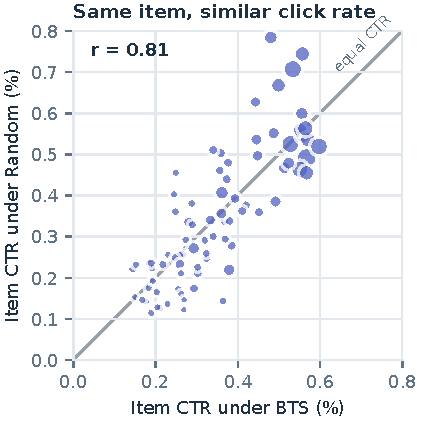
\includegraphics[width=\linewidth,height=.62\textheight,keepaspectratio]{eda_item_ctr.pdf}
\column{.55\linewidth}
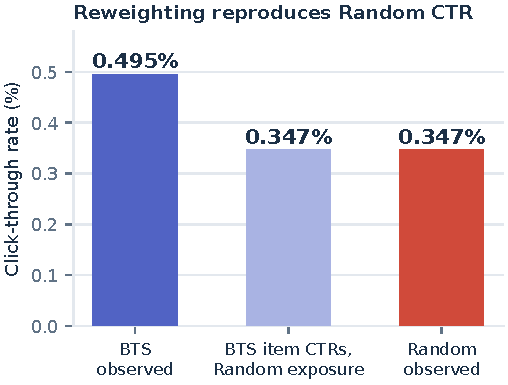
\includegraphics[width=\linewidth,height=.55\textheight,keepaspectratio]{eda_ctr_decomposition.pdf}\par
\aside{Middle bar: each item's BTS click rate, weighted by Random's uniform item mix.}
\end{columns}
\take{Reweighting BTS item click rates by Random's exposure reproduces Random's CTR: exposure mix explains most of the aggregate gap.}
\end{frame}

% ---------------------------------------------------------------- 6 PREPROCESSING / data check
\begin{frame}{Pre-processing \textperiodcentered{} One user segment has a different label in each log}
\begin{columns}[T,onlytextwidth]
\column{.50\linewidth}
\vspace{.15cm}
\begin{tabular}{@{}c@{\hspace{.7cm}}c@{}}
{\fontsize{26}{28}\selectfont\bfseries\color{bts}\profShareB\%} & {\fontsize{26}{28}\selectfont\bfseries\color{rnd}\profShareR\%}\\[.1cm]
\parbox{3.1cm}{\centering\footnotesize of BTS rows carry a profile never seen in Random} & \parbox{3.1cm}{\centering\footnotesize of Random rows carry a profile never seen in BTS}
\end{tabular}\par\vspace{.3cm}
\footnotesize
\begin{itemize}\setlength{\itemsep}{2pt}
\item Each of the 4 user features has exactly \emph{one} new code, and all four always occur together
\item Both segments click more than their log's average (\profLiftB\(\times\) / \profLiftR\(\times\))
\item Impressions were randomised, so both logs should share one user mix. Our inference (not documented): the same segment under a different code. Hence every result is also reported on matched-code rows
\end{itemize}
\column{.46\linewidth}
\sect{Why it matters}
\footnotesize With a standard ``unseen \(\to\) UNKNOWN'' encoding, the UNKNOWN coefficient is never trained. Our first pass predicted \textbf{\naivePred\%} CTR for this segment (observed \profCTRR\%) and \textbf{exaggerated the apparent cross-policy context penalty \(\sim\)\naiveRatio\(\times\)}.\par\vspace{.2cm}
\sect{What we did}
\footnotesize\begin{itemize}\setlength{\itemsep}{1pt}
\item Main analysis: map the Random-only profile to the BTS-only profile, using feature codes only, never Random clicks
\item Robustness: matched-code rows only, no mapping assumption (backup)
\item One-hot encode all six categorical predictors
\item Drop logged propensities \& affinity scores: they encode the policy itself
\end{itemize}
\end{columns}
\end{frame}

% ---------------------------------------------------------------- 7 DESIGN
\begin{frame}{Design \textperiodcentered{} Fit and tune on BTS; Random only evaluates}
\vspace{.2cm}
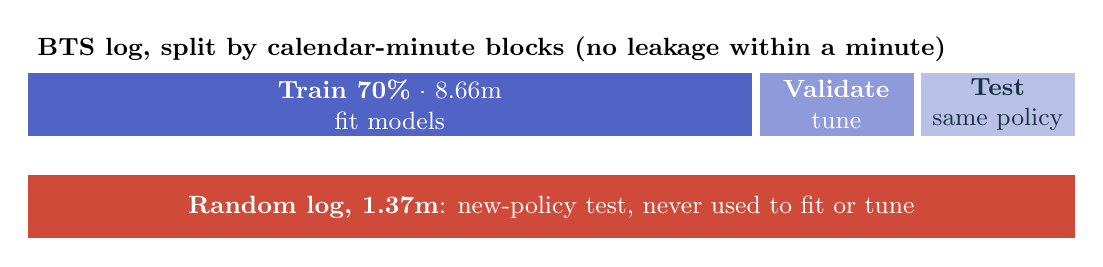
\begin{tikzpicture}[x=1cm,y=1cm,>=Latex]
\node[anchor=west,font=\small\bfseries] at (0,2.55) {BTS log, split by calendar-minute blocks (no leakage within a minute)};
\fill[bts] (0,1.45) rectangle (9.2,2.25);   \node[text=white,align=center,font=\small] at (4.6,1.85) {\textbf{Train 70\%} \textperiodcentered{} 8.66m\\fit models};
\fill[bts!65] (9.3,1.45) rectangle (11.25,2.25); \node[text=white,align=center,font=\small] at (10.27,1.85) {\textbf{Validate}\\tune};
\fill[bts!40] (11.35,1.45) rectangle (13.3,2.25); \node[text=ink,align=center,font=\small] at (12.32,1.85) {\textbf{Test}\\same policy};
\fill[rnd] (0,.15) rectangle (13.3,.95); \node[text=white,font=\small] at (6.65,.55) {\textbf{Random log, 1.37m}: new-policy test, never used to fit or tune};
\end{tikzpicture}
\vspace{.3cm}
\begin{columns}[T,onlytextwidth]
\column{.31\linewidth}
\sect{Metric}
\textbf{Log loss}: a proper scoring rule for click probabilities. AUC and calibration as checks.
\column{.31\linewidth}
\sect{Yardsticks}
\textbf{Constant CTR} and a smoothed \textbf{item\(\times\)position CTR table}. Gains are reported over the constant.
\column{.31\linewidth}
\sect{Uncertainty}
\textbf{Paired bootstrap} over minute blocks within each day (1{,}000 draws) \(\Rightarrow\) 95\% intervals.
\end{columns}
\end{frame}

% ---------------------------------------------------------------- 8 METHODS
\begin{frame}{Methods \textperiodcentered{} Three learners, from rigid to flexible}
\vspace{.1cm}
\begin{columns}[T,onlytextwidth]
\column{.31\linewidth}
{\large\color{teal}\bfseries Ridge logistic}\par\vspace{.1cm}
\small Additive log-odds; L2 penalty shrinks coefficients.\par\vspace{.15cm}
\aside{Tuned:} \(C \in 10^{-3},\dots,10^{3}\)\par
\aside{Selected:} \(C=\ridgeC\) \aside{(curve flat for \(C\ge 1\): with 8.7m rows the penalty barely binds)}
\column{.31\linewidth}
{\large\color{amber}\bfseries Pruned tree (CART)}\par\vspace{.1cm}
\small Gini splits, grown deep then \textbf{cost-complexity pruned} (\(\alpha_{\mathrm{ccp}}\)).\par\vspace{.15cm}
\aside{Tuned:} 25 pruning levels \(\times\) 2 min.\ leaf sizes \(\times\) 3 smoothing strengths\par
\aside{Selected:} \cartLeaves{} leaves \aside{(interior of 5--10{,}183)}
\column{.31\linewidth}
{\large\color{plum}\bfseries Random forest}\par\vspace{.1cm}
\small \forestB{} bootstrapped trees, random feature subset at each split; probabilities averaged.\par\vspace{.15cm}
\aside{Tuned:} features per split \(\times\) leaf size (\forestGrid{} configs)\par
\aside{Selected:} \forestMf\% of features, \forestLeafText
\end{columns}
\vspace{.15cm}
\begin{block}{Variable selection: every method fitted twice}
\textbf{item + position} \quad vs. \quad \textbf{item + position + 4 user features}. Does user context earn its place, and does it still earn it after the switch?
\end{block}
\vspace{.1cm}
\aside{All hyper-parameters chosen by BTS-validation log loss. Leaf click rates are shrunk towards the overall CTR, so no prediction is exactly 0. Exact fitting on 61k aggregated cells makes full-data training feasible.}
\end{frame}

% ---------------------------------------------------------------- 9 RESULT 1
\begin{frame}{Result 1 \textperiodcentered{} Flexible models win on BTS; after the switch, no clear winner}
\vspace{.05cm}
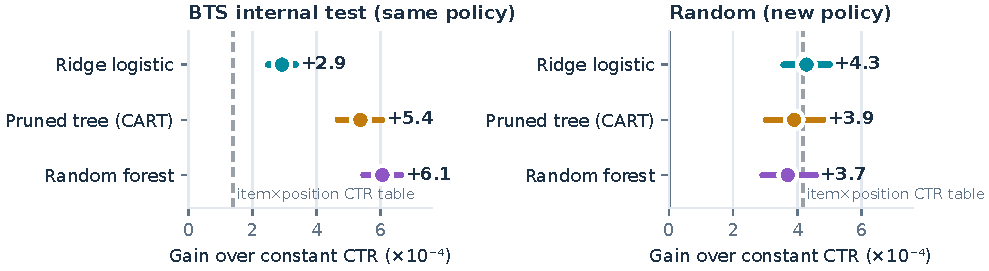
\includegraphics[width=\linewidth]{res_gains.pdf}
\vspace{-.1cm}
\begin{columns}[T,onlytextwidth]
\column{.48\linewidth}
\small\textbf{Same policy:} forest beats ridge by \hl{\fmrBTS} \aside{[\fmrBTSci]}, twice ridge's gain over the constant.
\column{.48\linewidth}
\small\textbf{New policy:} forest vs.\ ridge \hl{\fmrRND} \aside{[\fmrRNDci]}: the order flips numerically, but the 95\% interval includes 0. A plain item\(\times\)position CTR table does as well as any model.
\end{columns}
\take{The clear BTS ranking is not confirmed under the new policy.}
\end{frame}

% ---------------------------------------------------------------- 10 RESULT 2
\begin{frame}{Result 2 \textperiodcentered{} User context drove the BTS gains, but they did not carry over}
\vspace{.05cm}
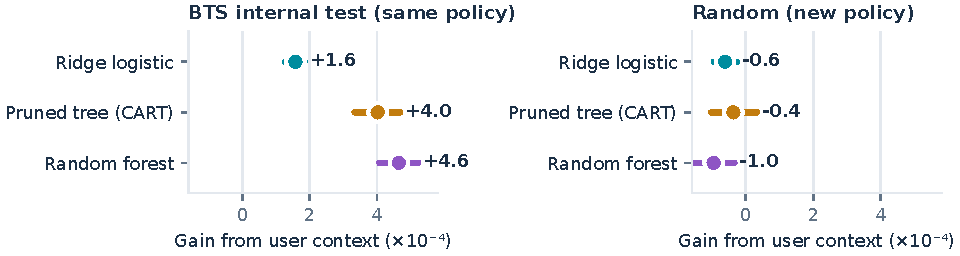
\includegraphics[width=\linewidth,height=.47\textheight,keepaspectratio]{res_context.pdf}
\vspace{-.05cm}
\begin{columns}[T,onlytextwidth]
\column{.48\linewidth}
\small On BTS, user features deliver \textbf{most of the trees' advantage} (\ctxCartB{} and \ctxForestB).
\column{.48\linewidth}
\small On Random, the same features make every model \textbf{slightly worse} (\ctxRangeR; interval excludes 0 for ridge and forest). Matched-code rows only: \ctxRangeSeen.
\end{columns}
\take{Here, gains from user features (additive in ridge, interactions in trees) did not carry over.}

\end{frame}

% ---------------------------------------------------------------- 11 RESULT 3
\begin{frame}{Result 3 \textperiodcentered{} More data improves every model, but gaps close after the switch}
\vspace{-.05cm}
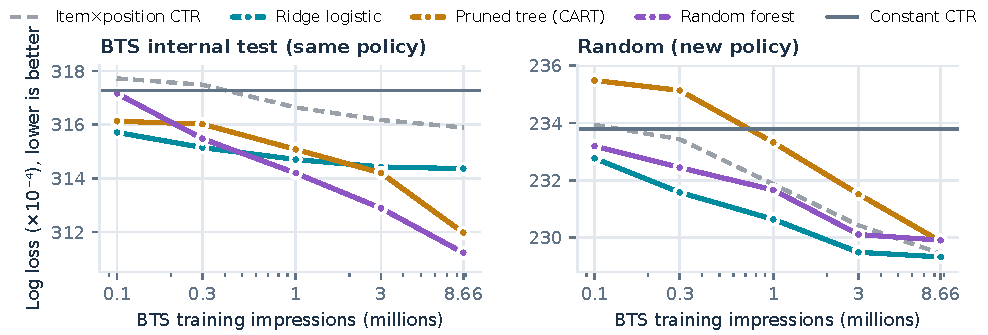
\includegraphics[width=\linewidth,height=.52\textheight,keepaspectratio]{res_curve.pdf}
\vspace{-.05cm}
\begin{columns}[T,onlytextwidth]
\column{.48\linewidth}
\small\textbf{Same policy:} \curveBTStext
\column{.48\linewidth}
\small\textbf{New policy:} \curveRNDtext
\end{columns}
\take{More old-policy data improved every model on Random, but did not restore the flexible models' BTS advantage.}
\end{frame}

% ---------------------------------------------------------------- 12 FINAL MODEL
\begin{frame}{Final model \textperiodcentered{} The random forest, before and after the switch}
\vspace{-.05cm}
\begin{columns}[T,onlytextwidth]
\column{.46\linewidth}
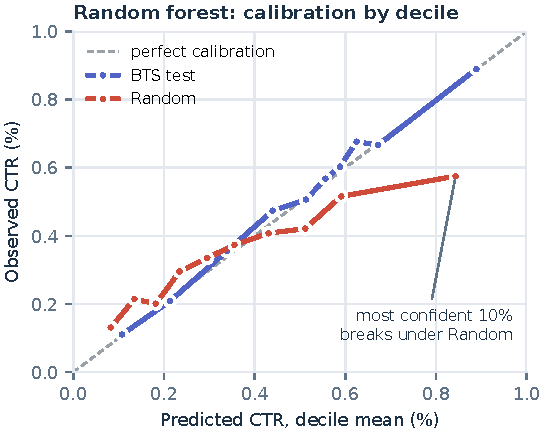
\includegraphics[width=\linewidth,height=.74\textheight,keepaspectratio]{res_calibration.pdf}
\column{.51\linewidth}
\sect{Selected by protocol: lowest BTS-validation loss}
\renewcommand{\arraystretch}{1.15}
\begin{tabular}{@{}lrr@{}}
& \color{bts}\textbf{BTS} & \color{rnd}\textbf{Random}\\\midrule
Log loss & \finLLB & \finLLR\\
vs.\ constant & \finSkillB\% & \finSkillR\%\\
AUC & \finAUCB & \finAUCR\\\bottomrule
\end{tabular}\par\vspace{.15cm}
\footnotesize
\begin{itemize}\setlength{\itemsep}{2pt}
\item \textbf{Anticipates the CTR drop}: predicts \finMeanR\% on Random vs.\ \rndCTR\% observed (a constant model would say \btsCTR\%)
\item \textbf{But its most confident calls break}: top decile \finTopPredR\% predicted vs.\ \finTopObsR\%
\item \textbf{Loses to the simplest model after the switch}: vs.\ ridge on item + position, \finVsSimpleB{} on BTS but \hl{\finVsSimpleR} \aside{[\finVsSimpleRci]} on Random
\end{itemize}
\end{columns}
\end{frame}

% ---------------------------------------------------------------- 13 TAKEAWAYS
\begin{frame}{Implications for a marketplace that changes its recommender}
\vspace{.15cm}
\small\begin{enumerate}\setlength{\itemsep}{.18cm}
\item \textbf{Validate under the policy you will deploy.} The best model on old logs lost to the simplest one on the new policy. Keep a small randomised slice of traffic as the honest test set.
\item \textbf{Prefer simpler, transferable effects until contextual gains are validated under the deployment policy.} Here, a simple item-level model matched or beat the forest after the switch; add context back once new-policy data confirm it helps.
\item \textbf{Audit categorical codes across data sources.} One relabelled segment exaggerated the apparent context penalty \(\sim\)\naiveRatio\(\times\) in our first pass.
\end{enumerate}
\vspace{.12cm}
\begin{block}{Answers}
\textbf{Q1:} Mostly. The final model stays 1.6--1.9\% better than a constant on both logs and anticipates the CTR drop. \textbf{Q2:} In this experiment, item-level signal transferred and more data helped; the gains from flexibility and user context did not carry over.
\end{block}
\vspace{.05cm}
\aside{Scope: one shop, one week, anonymised features. Predicting clicks is not the same as valuing a policy (that needs off-policy evaluation).}
\end{frame}

{\setbeamercolor{background canvas}{bg=ink}
\begin{frame}[plain]
\vfill\centering
{\fontsize{28}{32}\selectfont\color{white}\bfseries Thank you}\par\vspace{.3cm}
{\large\color{white!75} Questions and discussion}\par\vspace{.6cm}
{\small\color{white!55} Backup slides follow: tuning, full results, robustness, encoding details, limitations}
\vfill
\end{frame}}

\appendix
% ================================================================ BACKUP
\begin{frame}{Backup \textperiodcentered{} Hyper-parameter tuning on BTS validation}
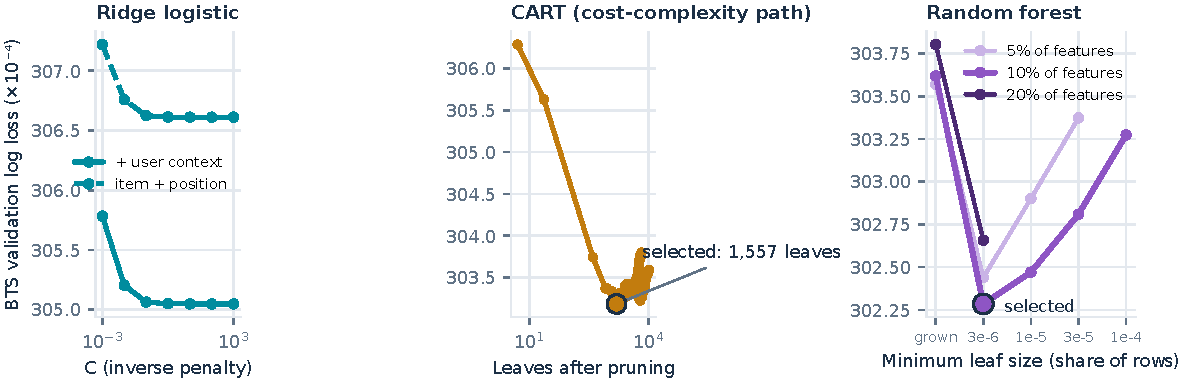
\includegraphics[width=\linewidth,height=.66\textheight,keepaspectratio]{bk_tuning.pdf}
\aside{Lower is better. Ridge: curve flat for \(C\ge 1\). CART: pruning path from 10{,}183 leaves down to 5; minimum in the interior. Forest: shown for the three feature fractions tested at every leaf size (full 21-configuration grid in the archive); optimum interior on both axes, 10\% of features and minimum leaf \(\approx\)26 impressions. 100 trees per grid cell; final model 300.}
\end{frame}

\begin{frame}{Backup \textperiodcentered{} All models, both logs}
\centering\small
\begin{tabular}{@{}llrrr@{\hspace{.6cm}}rrr@{}}\toprule
 & & \multicolumn{3}{c}{\color{bts}\textbf{BTS test}} & \multicolumn{3}{c}{\color{rnd}\textbf{Random}}\\
Model & Features & Log loss & AUC & Mean pred. & Log loss & AUC & Mean pred.\\
 & & \(\times10^{4}\) & & \% & \(\times10^{4}\) & & \%\\\midrule
Constant CTR &  & 317.28 & 0.500 & 0.495 & 233.62 & 0.500 & 0.495 \\
Item\(\times\)position CTR &  & 315.89 & 0.557 & 0.498 & 229.45 & 0.591 & 0.374 \\
Ridge logistic & item+pos & 315.94 & 0.556 & 0.494 & 228.72 & 0.607 & 0.349 \\
Ridge logistic & + user & 314.36 & 0.597 & 0.494 & 229.33 & 0.608 & 0.348 \\
CART (pruned) & item+pos & 315.93 & 0.557 & 0.494 & 229.34 & 0.595 & 0.355 \\
CART (pruned) & + user & 311.91 & 0.619 & 0.484 & 229.71 & 0.622 & 0.338 \\
Random forest & item+pos & 315.87 & 0.558 & 0.495 & 228.96 & 0.602 & 0.352 \\
Random forest & + user & 311.22 & 0.624 & 0.493 & 229.91 & 0.610 & 0.366 \\
\bottomrule\end{tabular}
\par\vspace{.2cm}
\aside{BTS test: 1{,}846{,}068 impressions; Random: 1{,}374{,}327 (harmonised profile). Mean pred.\ = average predicted CTR; observed CTR \btsTestCTR\% / \rndCTR\%.}
\end{frame}

\begin{frame}{Backup \textperiodcentered{} Paired bootstrap contrasts (\(\times 10^{-4}\) log loss)}
\centering\small
\begin{tabular}{@{}lrlrl@{}}\toprule
Contrast (A \(-\) B) & \multicolumn{2}{c}{\color{bts}\textbf{BTS test}} & \multicolumn{2}{c}{\color{rnd}\textbf{Random}}\\\midrule
Constant \(-\) Ridge logistic (+ user) & +2.92 & [+2.49, +3.36] & +4.29 & [+3.58, +5.01] \\
Constant \(-\) CART (pruned) (+ user) & +5.37 & [+4.67, +6.04] & +3.91 & [+3.03, +4.81] \\
Constant \(-\) Random forest (+ user) & +6.06 & [+5.47, +6.63] & +3.71 & [+2.92, +4.57] \\
\midrule
Ridge \(-\) Forest (both + user) & +3.13 & [+2.55, +3.74] & \(-\)0.58 & [\(-\)1.28, +0.12] \\
Ridge \(-\) CART (both + user) & +2.45 & [+1.81, +3.11] & \(-\)0.38 & [\(-\)1.05, +0.24] \\
CART \(-\) Forest (both + user) & +0.69 & [+0.33, +1.10] & \(-\)0.20 & [\(-\)0.82, +0.45] \\
Ridge item+pos \(-\) Forest + user (final) & +4.71 & [+4.13, +5.28] & \(-\)1.20 & [\(-\)1.80, \(-\)0.58] \\
\midrule
Ridge logistic: item+pos \(-\) + user & +1.58 & [+1.27, +1.85] & \(-\)0.61 & [\(-\)0.95, \(-\)0.26] \\
CART (pruned): item+pos \(-\) + user & +4.02 & [+3.34, +4.68] & \(-\)0.37 & [\(-\)1.03, +0.33] \\
Random forest: item+pos \(-\) + user & +4.65 & [+4.07, +5.22] & \(-\)0.95 & [\(-\)1.56, \(-\)0.34] \\
\bottomrule\end{tabular}
\par\vspace{.2cm}
\aside{Difference A \(-\) B in mean log loss; positive = B better. 1{,}000 resamples of calendar-minute blocks within each day; intervals are conditional on the fitted models.}
\end{frame}

\begin{frame}{Backup \textperiodcentered{} Robustness: matched-code rows vs.\ relabelled segment}
\centering\small
\begin{tabular}{@{}lrrr@{\hspace{.6cm}}rrr@{}}\toprule
 & \multicolumn{3}{c}{Matched-code rows (888{,}334)} & \multicolumn{3}{c}{Relabelled segment (485{,}993)}\\
Log loss \(\times10^{4}\) & item+pos & + user & gain & item+pos & + user & gain\\\midrule
Ridge logistic & 216.61 & 217.63 & \(-\)1.02 & 250.85 & 250.72 & +0.13 \\
CART (pruned) & 217.35 & 218.07 & \(-\)0.72 & 251.27 & 251.00 & +0.27 \\
Random forest & 216.93 & 217.06 & \(-\)0.13 & 250.96 & 253.41 & \(-\)2.46 \\
\bottomrule\end{tabular}\par\vspace{.15cm}
{\footnotesize\color{muted} Context-gain 95\% CIs on matched rows: ridge [\(-\)1.59, \(-\)0.48], CART [\(-\)1.76, +0.31], forest [\(-\)0.93, +0.71].}
\par\vspace{.25cm}
\raggedright\small
\begin{itemize}
\item On matched-code rows (no mapping assumption), adding user context never helps any method: \ctxRangeSeen{} vs.\ \(+1.6\) to \(+4.6\) on BTS.
\item On the relabelled segment the effect is small for ridge and CART and negative for the forest.
\end{itemize}
\end{frame}

\begin{frame}{Backup \textperiodcentered{} What the naive encoding did}
\small
\begin{columns}[T,onlytextwidth]
\column{.5\linewidth}
\sect{Mechanism}
\begin{itemize}\setlength{\itemsep}{3pt}
\item One-hot with an UNKNOWN column per feature, fitted on BTS training data \(\Rightarrow\) UNKNOWN is never 1 in training \(\Rightarrow\) its coefficient stays 0.
\item Full one-hot plus an unpenalised intercept: with weak shrinkage (\(C=10\)) the intercept drifts to \(-3.03\) while every user level gets a compensating negative coefficient.
\item An all-UNKNOWN row keeps the intercept but loses the compensation \(\Rightarrow\) predicted CTR \naivePred\% vs.\ \profCTRR\% observed.
\end{itemize}
\column{.46\linewidth}
\sect{Effect on the context contrast (ridge, Random)}
\renewcommand{\arraystretch}{1.25}
\begin{tabular}{@{}lr@{}}
\toprule
Encoding & M1 \(-\) M2 \((\times10^{-4})\)\\\midrule
Naive UNKNOWN & \naiveDiff\\
Harmonised profile & \ctxRidgeR\\
Matched-code rows only & \ctxRidgeSeen\\\bottomrule
\end{tabular}\par\vspace{.3cm}
\aside{Evidence for ``same segment, relabelled'': exactly one new code per feature, all four co-occurring; mirror profile in BTS with equal share (35.3\% vs 35.4\%); both click above their log's average.}
\end{columns}
\end{frame}

\begin{frame}{Backup \textperiodcentered{} Learning curves in numbers}
\centering\small
\begin{tabular}{@{}lrrrrr@{}}\toprule
Training rows & 0.1m & 0.3m & 1m & 3m & 8.66m\\\midrule
\multicolumn{6}{@{}l}{\textbf{BTS test}}\\
Constant CTR & 317.28 & 317.27 & 317.28 & 317.28 & 317.28 \\
Item\(\times\)position CTR & 317.72 & 317.48 & 316.64 & 316.17 & 315.89 \\
Ridge logistic & 315.71 & 315.14 & 314.70 & 314.42 & 314.36 \\
CART (pruned) & 316.12 & 316.02 & 315.07 & 314.20 & 311.97 \\
Random forest & 317.15 & 315.48 & 314.19 & 312.88 & 311.22 \\
\multicolumn{6}{@{}l}{\textbf{Random}}\\
Constant CTR & 234.05 & 233.99 & 233.60 & 233.67 & 233.62 \\
Item\(\times\)position CTR & 233.93 & 233.43 & 231.86 & 230.43 & 229.45 \\
Ridge logistic & 232.77 & 231.58 & 230.64 & 229.49 & 229.33 \\
CART (pruned) & 235.48 & 235.13 & 233.32 & 231.52 & 229.87 \\
Random forest & 233.19 & 232.44 & 231.66 & 230.11 & 229.91 \\
\bottomrule\end{tabular}
\par\vspace{.2cm}
\aside{Nested training prefixes of a randomised calendar-minute order; every method re-tuned on BTS validation at every size. Log loss \(\times 10^{4}\). All three methods and the item\(\times\)position table improve at every step on both logs; the constant baseline only varies with each subsample's CTR.}
\end{frame}

\begin{frame}{Backup \textperiodcentered{} What drives predictions}
\begin{columns}[T,onlytextwidth]
\column{.48\linewidth}
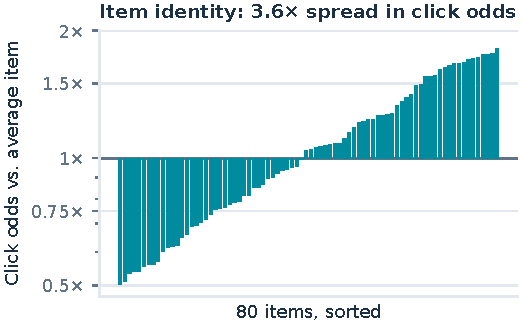
\includegraphics[width=\linewidth]{res_items.pdf}\par
\aside{Ridge (item + position): odds ratios relative to the average item. Position odds ratios: \posORs.}
\column{.48\linewidth}
\sect{Permutation importance (\(\times10^{-4}\) log loss)}
\small\begin{tabular}{@{}lrrrr@{}}\toprule
 & \multicolumn{2}{c}{Ridge + user} & \multicolumn{2}{c}{Forest + user}\\
Group & BTS & Random & BTS & Random\\\midrule
item & 2.83 & 5.13 & 9.42 & 7.50 \\
position & -0.01 & 0.00 & 1.93 & 0.04 \\
user profile & 3.67 & 0.56 & 10.48 & 4.37 \\
\bottomrule\end{tabular}\par\vspace{.2cm}
\aside{Increase in log loss when one feature group is shuffled across rows. Permuting user features creates profile--item combinations the trees never saw, so importance stays positive on Random even though dropping the features costs nothing (Result 2).}
\end{columns}
\end{frame}

\begin{frame}{Backup \textperiodcentered{} Implementation details}
\small
\begin{itemize}\setlength{\itemsep}{4pt}
\item \textbf{Exact aggregation.} Six categorical predictors \(\Rightarrow\) every impression is one of 61{,}555 BTS patterns. Each pattern enters as two weighted rows (clicks, non-clicks): identical log-likelihood, Gini impurity and pruning path as the 8.66m raw rows.
\item \textbf{Forest bootstrap.} Poisson(1) resampling of each pattern's clicks and non-clicks: the standard large-\(n\) equivalent of drawing \(n\) rows with replacement.
\item \textbf{Leaf smoothing.} Leaf CTR \(=(\text{clicks}+m\,\bar p)/(\text{impressions}+m)\), \(m\) tuned (CART) or fixed at 100 (forest), so that no leaf predicts exactly 0.
\item \textbf{Split.} 70/15/15 by calendar-minute blocks within each day (seed 20261114); no deduplication.
\item \textbf{Software.} Python, scikit-learn (\texttt{LogisticRegression}, \texttt{DecisionTreeClassifier} with \texttt{ccp\_alpha}, the scikit-learn counterpart of rpart's \texttt{cp} used in class). Code and numerical outputs available upon request.
\end{itemize}
\end{frame}

\begin{frame}{Backup \textperiodcentered{} Limitations}
\small
\begin{itemize}\setlength{\itemsep}{5pt}
\item \textbf{One shop, one week, one A/B test.} Results describe this shift (adaptive \(\to\) uniform), not every policy change.
\item \textbf{Anonymised features.} The relabelled-profile mapping is an inference from shares and co-occurrence, not documented; matched-code results do not depend on it.
\item \textbf{Prediction \(\ne\) policy value.} We test whether click probabilities transfer, not which policy earns more clicks (that needs off-policy evaluation, e.g.\ inverse propensity weighting).
\item \textbf{Exploratory use of Random.} Our first-pass analysis looked at Random results; that is how the encoding problem was found. The corrected pipeline makes every choice on BTS, but Random is not an untouched, pre-registered holdout.
\item \textbf{Natural fix not tried:} re-weighting BTS training rows by \(1/\text{propensity}\) to mimic uniform exposure; the logged propensities make this the next experiment.
\item \textbf{Intervals} treat minute blocks as independent and condition on the fitted models (no refitting inside the bootstrap).
\end{itemize}
\end{frame}

\begin{frame}{Backup \textperiodcentered{} References}
\small
\begin{itemize}\setlength{\itemsep}{5pt}
\item Saito, Aihara, Matsutani, Narita (2021). \emph{Open Bandit Dataset and Pipeline: Towards Realistic and Reproducible Off-Policy Evaluation.} NeurIPS Datasets \& Benchmarks; arXiv:2008.07146.
\item James, Witten, Hastie, Tibshirani. \emph{An Introduction to Statistical Learning}: logistic regression, regularisation, tree-based methods.
\item Hastie, Tibshirani, Friedman. \emph{The Elements of Statistical Learning}: model assessment, random forests.
\item Breiman, Friedman, Olshen, Stone (1984). \emph{Classification and Regression Trees} (cost-complexity pruning).
\item Course materials: Statistical and Machine Learning, WU Vienna (2026), units 04--06.
\end{itemize}
\end{frame}

\end{document}
